\documentclass{article}
\usepackage{amssymb}
\usepackage{amsmath}
\usepackage{mathtools}
\usepackage{cancel}
\usepackage{tikz}
\usepackage{hyperref}
\usepackage{circuitikz}
\usepackage{float}
\usepackage{afterpage}
\usepackage{pgfplots}
\usepackage{textcomp}
\usepgfplotslibrary{groupplots}
\usetikzlibrary{calc, arrows}
\newtheorem{theorem}{Theorem}
\newtheorem{definition}{Definition}
\newtheorem{corollary}{Corollary}
\newtheorem{proof}{Proof}
\tikzstyle{int}=[draw, fill=blue!20, minimum size=2em]
\tikzstyle{init} = [pin edge={to-,thin,black}]

\tikzstyle{block} = [draw, fill=blue!20, rectangle, 
    minimum height=3em, minimum width=6em]
\tikzstyle{sum} = [draw, fill=blue!20, circle, node distance=1cm]
\tikzstyle{input} = [coordinate]
\tikzstyle{output} = [coordinate]
\tikzstyle{pinstyle} = [pin edge={to-,thin,black}]

\DeclareMathOperator*{\argmin}{argmin}

\begin{document}
\title{EE123 Course Notes}
\author{Anmol Parande}
\date{Spring 2020 - Professor Miki Lustig}
\maketitle
\textbf{Disclaimer: }These notes reflect EE123 when I took the course (Spring 2020). They may not accurately reflect current course content, so use at your own risk.
If you find any typos, errors, etc, please raise an issue on the \href{https://github.com/parandea17/BerkeleyNotes}{GitHub repository}.\\
\tableofcontents
\newpage
\section{The DFT}
Whereas the CTFT takes a continuous signal and outputs a continuous frequency spectrum and the DTFT takes a discrete signal
and outputs a continuous, periodic frequecy spectrum, the Discrete Fourier Transform takes a discrete finite signal and outputs
a discrete frequency spectrum. This is useful for signal processing because we cannot store infinite signals in a computers memory.
\begin{definition}
    For a length $N$ finite sequence $\{x[n]\}^{n-1}_{0}$, the Discrete Fourier Transform of the signal
    is a length N finite sequence $\{X[k]\}^{n-1}_{0}$ where
    $$X[k] = \sum_{n=0}^{N-1}{x[n]e^{-j\frac{2\pi}{N}kn}}$$
\end{definition}
One way to interpret the DFT is in terms of the Fourier series for a disrete periodic signal $\tilde{x}[n]=x[((n))_N]$. Recall that the coefficient of the kth term of the Fourier Series is
$$a_k = \frac{1}{N}\sum_{n=0}^{N-1}{x[n]e^{-j\frac{2\pi}{N}kn}}$$
Notice that the $a_k$ of the Fourier Series are the DFT values except scaled by a factor of $N$. This gives an intuitive inverse DFT.
\begin{definition}
    For a length N finite sequence $\{X[k]\}^{N-1}_{0}$ representing the DFT of a finite perioidc signal $\{x[n]\}^{N-1}_{0}$,
    the inverse DFT is given by
    $$x[n] = \frac{1}{N}\sum_{k=0}^{N-1}{X[k]e^{j\frac{2\pi}{N}kn}}$$
\end{definition}
Notice that the DFT and the IDFT are very similar in form. It turns out that the IDFT can be expressed as a DFT of $X^*[k]$. Namely
$$IDFT\{X[k]\} = \frac{1}{N}DFT\{X^\star[k]\}^\star$$
Further intuition for the DFT comes from relating it to the DTFT. Suppose we have a finite signal $x[n]$ which is $0$ for $n < 0$ and $n > N-1$.
The DTFT of this signal is
$$X(\omega) = \sum_{n=-\infty}^{\infty}{x[n]e^{-j\omega n}} = \sum_{n=0}^{N-1}{x[n]e^{-j\omega n}}$$
Suppose we sample the DTFT at intervals of $\frac{2\pi}{N}k$, then
$$X[k] = X\left(\frac{2\pi}{N}k\right) = \sum_{n=0}^{N-1}{x[n]e^{-j\frac{2\pi}{N}k n}}$$
Thus we can think of the DFT as a $N$ point sample of the DTFT.
One important point to notice though is that while the DTFT is often centered around 0, because we are summing
from 0 to N-1 in the DFT, the DFT coefficients are centered around $\pi$.
\subsection{Convolution and the DFT}
\subsubsection{Circular Convolution}
When the DFT coefficients of two signals are multiplied, the resulting coefficients describe a circular convolution of the original two signals.
$$x[n]\circledast y[n] \leftrightarrow X[k]Y[k]$$
The circular convolution is defined as follows
$$x[n]\circledast y[n] = \sum_{m=0}^{N-1}x[m]y[((n-m))_N]$$
The mechanics of the circular convolution are the same as that of the regular convolution, except the signal is circularly shifted.
\begin{figure}[h!]
  \centering
  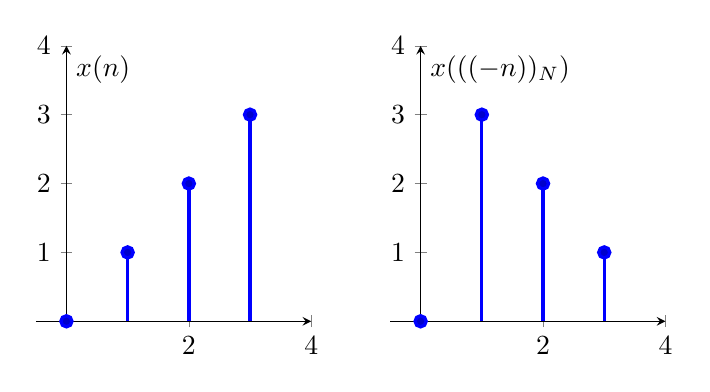
\begin{tikzpicture}
    \begin{groupplot}[
        group style={group size=2 by 1},
        axis lines=middle,
        width=2in,
        height=2in,
        ymax=4]
      \nextgroupplot[ylabel=$x(n)$, xmin=-0.5, xmax=4];
      \addplot+[ycomb, line width=1.2pt] plot coordinates {(0, 0) (1, 1) (2, 2) (3, 3)};
      \nextgroupplot[ylabel=$x(((-n))_N)$, xmin=-0.5, xmax=4];
      \addplot+[ycomb, line width=1.2pt] plot coordinates {(0, 0) (1, 3) (2, 2) (3, 1)};
    \end{groupplot}
  \end{tikzpicture}
  \caption{A circular shift}
\end{figure}
A circular convolution is equivalent to a periodic convolution over a single period.
\subsubsection{Linear Convolution with the DFT}
Because multiplying DFT coefficients performs a convolution, it turns out that we can compute a linear convolution using the circular convolution.
\begin{align*}
  x[n] \qquad 0\le n\le L-1\\
  h[n] \qquad 0 \le n \le P-1
\end{align*}
The linear convolution of these two signals will be length $L+P-1$, so in order to take an IDFT and get $L+P-1$ samples, we need to
take at least $N\le L+P-1$ points.
\begin{itemize}
  \item[1.] Pad each vector to length $L+P-1$
  \item[2.] Compute $X[k]H[k]$
  \item[3.] Take the Inverse DFT
\end{itemize}
If $N$ is too small, the result is akin to aliasing in the time domain.
To see why, consider that the DFT coefficients are essentially the DFS coefficients of the periodic extension of $x[n]$
$$\tilde{x}[n]=\sum_{r=-\infty}^{\infty}x[n-rN]$$
If we compute the DTFT of each periodic extension, then
$$Y(e^{j\omega})=X(e^{j\omega})H(e^{j\omega})$$ and the IDTFT of this will be
$$\tilde{y}[n] = \sum_{r=-\infty}^{\infty}y[n-rN]$$
Notice that if $N$ is not large enough, then these copies will be overlapping (a.k.a aliasing).
Since the DFT is just sampling the DTFT, the circular convolution will represent the true convolution
so long as the copies don't overlap.
\subsubsection{Block Convolutions}
In a discrete time system, the input signal might have a very long length, making it impractical to be stored in a computer's memory
or to compute the DFT of it all at once (especially if we have a real-time system). To compute the output of the filter (with impulse response of length $P$), we need to compute
the DFT in blocks shorter than the signal. \\\\The first method of block convolution is the overlap-add method.
\begin{itemize}
  \item[1.] Decompose $x[n]$ into nonoverlapping segments of length $L$
  \[ x_r[n] =
    \begin{cases}
      x[n] & rL \le n \le (r+1)L\\
      0 & \text{else}
    \end{cases}
  \]
  $$x[n] = \sum_{r}x_r[n]$$
  \item[2.] Since convolution is linear
  $$y[n] = x[n]*h[n]=\sum_r{x_r[n]*h[n]}$$
  \item[3.] Zero pad $x_r[n]$ and $h[n]$ to length $N\ge L+P-1$
  \item[4.] Compute the DFTs, multiply them, and take the inverse.
  \item[5.] The neighboring outputs overlap $P-1$, add the overlapping sections together to get the final output  
\end{itemize}
The other method of block convolution is the overlap-save method.
\begin{itemize}
  \item[1.] Divide $x[n]$ into sections of length $L$ such that each section overlaps the previous by $P-1$ points
  $$x_r[n]=x[n+r(L-P+1)-P+1] \qquad 0 \le n \le L-1$$
  \item[2.] Zero pad $x_r[n]$ and $h[n]$ to length $N\ge L+P-1$
  \item[3.] Compute the DFTs, multiply the coefficients, and compute the inverse.
  \item[4.] The first $P-1$ samples of the output will be incorrect, so we can discard them.
  $$y[n]=\sum_{r=0}^{\infty}y_r[n-r(L-P+1)+P-1]$$
  \[
    y_r[n]=
    \begin{cases}
      x_r[n]*h[n] & P-1\le n \le L-1\\
      0 & \text{ else}
    \end{cases}
  \]
\end{itemize}
\subsection{FFT}
The DFT gives us an easy way to do convolutions. Unfortunately, computing it is an $O(N^2)$ operation
because we must sum together $N$ elements to compute $N$ different coefficients. Thankfully, there is a fast
algorithm which can compute the DFT in $O(N\log N)$ time so we can compute convolutions quickly. The \textbf{Fast Fourier Transform}
is the algorithm which enables us to compute the DFT efficiently by exploiting properties of the Nth roots of unity.
$$W_N=e^{-j\frac{2\pi}{N}}$$
The roots of unity have the following properties:
\begin{align*}
  \textbf{Conjugate Symmetry: }& W_N^{N-n} = W_N^{-kn} = (W_N^{kn})^\star\\
  \textbf{Periodicity in N: }& W_{kn} = W_N^{k(n+N)} = W_N^{(k+N)n}\\
  \textbf{Power: } & W_N^2 = W_\frac{N}{2}
\end{align*}
There are two approaches to the FFT: decimation in time, which splits $x[n]$ into smaller subsequences, and decimation in frequency
which splits $X[n]$ into smaller subsequences.
\subsubsection{Decimation in Time}
The idea here is too break $x[n]$ into smaller subsequences. We assume that $N$ is a power of 2 for simplicity.
\begin{align*}
  X[k]=\sum_{n=0}^{N-1}x[n]W_N^{kn} = \sum_{\text{n even}}x[n]W_N^{kn}+\sum_{\text{n odd}}x[n]W_N^{kn}
\end{align*}
We let $n=2r$ and $n=2r+1$.
\begin{align*}
  X[k] &= \sum_{r=0}^{\frac{N}{2}-1}x[2r]W_N^{2rk}+\sum_{r=0}^{\frac{N}{2}-1}x[2r+1]W_N^{k(2r+1)}\\
  &= \sum_{r=0}^{\frac{N}{2}-1}x[2r]W_{\frac{N}{2}}^{rk}+W_N^k\sum_{r=0}^{\frac{N}{2}-1}x[2r+1]W_{\frac{N}{2}}^{kr}\\
\end{align*}
These are just the DFTs of the even and odd elements of the signal!
\begin{align*}
  \therefore X[k] = G[k] + W_N^kH[k]
\end{align*}
Both $G$ and $H$ are $\frac{N}{2}$ periodic, and notice that
$$W_N^{k+\frac{N}{2}}=e^{-j\frac{2\pi}{N}(k+\frac{N}{2})}= -W_N^k$$
This means once we compute $G[k]$ and $H[k]$ we can compute $X[k]$ easily because
$$X[k] = G[k]+W_N^kH[k]\qquad X\left[k+\frac{N}{2}\right]=G[k]-W_N^kH[k] \qquad \text{for }k\in\left[0, \frac{N}{2}\right)$$
We can continue this relationship recursively downwards.
Once we get too $N=2$, we can represet this as a simple butterfly operation.
$$X[0] = x[0]+x[1] \qquad X[1] = X[0]-X[1]$$
\subsubsection{Decimation in Frequency}
The decimation in frequency approach is very similar to the decimation in time approach except instead we split the frequency components
\begin{align*}
  X[2r] &= \sum_{n=0}^{\frac{N}{2}-1}x[n]W_N^{2rn}+\sum_{n=0}^{\frac{N}{2}-1}x\left[n+\frac{N}{2}\right]W_N^{2r\left(n+\frac{N}{2}\right)}=W_{\frac{N}{2}}^{rn}\sum_{n=0}^{\frac{N}{2}-1}\left(x[n]+x\left[n+\frac{N}{2}\right]\right)\\
  X[2r+1] &= W_{\frac{N}{2}}^{rn}\sum_{n=0}^{\frac{N}{2}-1}\left(x[n]-x\left[n+\frac{N}{2}\right]\right)
\end{align*}
\end{document}